\chapter{面向疾病传播控制：大规模移动对象上的连续暴露发现}

\section{引言}
传染性疾病长期以来一直被视为重大的公共卫生问题。密切接触发现（close contact discovery）在防止疫情传播方面发挥着不可或缺的作用。在此背景下，我们研究\textbf{连续暴露搜索问题}：给定一组移动对象和一组移动查询对象，在一段时间内持续地发现所有直接或间接暴露于至少一个查询对象的对象。

该问题面向多种应用场景，包括但不限于疾病防控、疫情预警、信息传播分析以及共移动模式挖掘。

为了解决该问题，我们设计了一种带有优化策略的精确群组处理算法。此外，我们还提出了一种近似算法，在不产生漏检（false dismissal）的前提下显著提升了计算效率。大量实验结果验证了所提出算法在有效性和效率方面的优势。
\subsection{研究背景与意义}
随着位置追踪设备（如车载导航系统和智能手机）以及 GPS 赋能服务（如 Google Maps）的持续普及，轨迹数据的规模正在迅速增长。在多种轨迹查询任务中~\cite{DBLP:conf/icde/ChenSJ0K20,DBLP:journals/vldb/ShangCWJZK18,DBLP:conf/ijcai/ChenSFK21,DBLP:journals/tkde/ShangCZJWK19}，接触搜索与接触追踪问题近年来受到了广泛关注~\cite{DBLP:journals/pvldb/Xu0B20,DBLP:conf/dasfaa/ChaoHLZ021,react}。一般而言，当两个移动对象在一段时间内保持较近的空间距离并相互影响时，即构成一次密切接触。对密切接触进行高效、准确的发现，在诸多实际场景中具有重要意义，包括但不限于疾病防控、疫情预警、信息传播分析以及共移动模式挖掘。在疫情期间，实时发现密切接触对象有助于限制人群传播并评估个体感染风险。

现有研究主要聚焦于针对单个查询对象（或查询轨迹）的接触追踪问题，通常基于查询对象与数据对象之间的空间邻近性进行处理（如~\cite{DBLP:conf/sigmod/FaloutsosRM94,DBLP:journals/pvldb/AssentWKKS09}），也有部分研究基于轨迹片段之间的相似性计算开展分析（如~\cite{DBLP:conf/icde/RongLSWLD17,DBLP:journals/pvldb/XieLP17}）。然而，在疾病暴发期间，大规模个体可能在短时间内被感染，因此，基于轨迹对海量移动对象进行连续接触搜索显得尤为重要。一个有效的接触搜索方法不仅需要能够同时处理大规模移动对象，还应保证对每个对象的实时检测能力。

据我们所知，现有研究通常将该问题建模为独立的查询处理问题、轨迹搜索问题~\cite{DBLP:journals/information/AlarabiBHA21,DBLP:conf/dasfaa/ChaoHLZ021}，或多查询搜索问题~\cite{DBLP:journals/corr/abs-2004-06653,DBLP:ptop}。这些方法要么仅适用于少量查询，要么假设输入为静态轨迹集合，因而在实际场景中难以有效处理大规模移动对象及大量查询。此外，这些方法也难以为每个对象持续维护实时检测结果。

\begin{figure}[t]
    \centering
    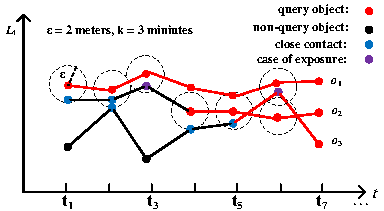
\includegraphics[width=0.8\textwidth]{fig/section5/intro.pdf}
    \caption{Example of cases of exposure}
    \label{fig:intro}
\end{figure}
\subsection{相关工作}
与我们研究的问题相似的一个方向是协同行为模式挖掘（co-movement pattern mining）。现有研究已经讨论了多种有趣的协同行为模式
\cite{DBLP:journals/pvldb/JeungYZJS08,DBLP:journals/pvldb/LiDHK10,flock,tang,DBLP:conf/icde/ZhengZYS13}。
其中，flock 模式 \cite{flock} 是最早提出的协同行为模式，用于刻画在连续 $k$ 个时间区间内共同移动的 $m$ 个移动对象组成的群体。
在相关工作中，文献 \cite{DBLP:conf/icde/ZhengZYS13} 从交通拥堵发现的角度提出了 gathering 模式。
此外，文献 \cite{tang} 以流式方式挖掘协同行为群体。
与上述研究不同的是，我们的 CES 问题不要求对群体中对象数量进行约束。
需要注意的是，在我们的定义下，群体之外的对象也可能被视为感染对象。
因此，这些研究提出的解决方案均无法直接应用于我们的问题。

为了有效防止 SARS、埃博拉以及 COVID-19 等传染病的传播，已有大量相关研究被提出
\cite{web,DBLP:journals/pvldb/Xu0B20,DBLP:journals/corr/abs-2004-06653}。
其中，文献 \cite{DBLP:journals/pvldb/Xu0B20} 首次提出了接触追踪（contact tracing）问题，
但该工作主要关注疾病传播的模拟，无法支持实时查询。
从另一个角度来看，文献 \cite{web} 提出了接触追踪查询（Contact Tracing Query, CTQ），
用于识别与查询对象存在直接或间接接触的个体。
文献 \cite{DBLP:conf/dasfaa/ChaoHLZ021} 提出了广义轨迹接触搜索（Trajectory Contact Search, TCS）查询，并设计了一种迭代算法进行求解。
另一项相关工作 \cite{DBLP:journals/information/AlarabiBHA21} 提出了一种用于追踪与患者接触的所有对象并搜索潜在感染者的技术，
但该方法基于轨迹片段，且主要面向室内应用场景。
据我们所知，现有方法均无法直接用于解决本文提出的问题，
因为它们要么针对静态轨迹数据，要么采用了不同的暴露案例定义。
\subsection{研究成果与贡献}

在此背景下，我们定义并研究了连续暴露搜索（Continuous Exposure Search，CES）问题：给定一组移动对象 $\mathcal{O}$，以及一个查询集合 $\mathcal{Q}\in\mathcal{O}$，用于表示已有的暴露病例，我们的目标是通过实时更新 $\mathcal{Q}$，持续检测新的暴露病例。在我们的设定中，新的暴露病例是指在距离阈值 $\epsilon$ 内、并且在时间阈值 $k$ 内与查询对象共同移动的对象。

如图 \ref{fig:intro} 所示的示例中，设 $o_1, o_2, o_3$ 为三个移动对象，初始查询集合为 $\mathcal{Q}=\{o_1\}$。距离阈值 $\epsilon$ 设为 2 米，接触时长阈值 $k$ 设为 3 分钟。我们使用红色、蓝色和紫色点分别表示已暴露（查询）对象的位置、密切接触对象的位置以及最新确认的暴露病例的位置。对象 $o_2$ 在连续时间段 $[t_1, t_3]$ 内与查询对象 $o_1$ 保持密切接触，因此我们将 $o_2$ 加入查询集合，即更新为 $\mathcal{Q}=\{o_1,o_2\}$，并在 $t_3$ 时刻返回更新后的 $\mathcal{Q}$ 作为实时结果。类似地，对象 $o_3$ 在时间段 $[t_4, t_6]$ 内与查询对象发生密切接触，因此在 $t_6$ 时刻将查询集合更新为 $\mathcal{Q}=\{o_1,o_2,o_3\}$。

为 CES 问题设计一种既高效又有效的解决方案并非易事。直接方法难以应对大规模移动对象，同时也无法保证实时性。为此，我们提出了一种高效的精确实时搜索算法，并引入多种优化技术。此外，我们还提出了一种近似实时搜索算法，在不产生漏检的前提下进一步提升搜索效率。本文的主要贡献总结如下：

\begin{itemize}
     \item 我们定义了一种新的 CES 问题，用于在大量移动对象中持续维护最新的暴露病例。该问题有助于监测和控制流行病的传播，例如 SARS、埃博拉和 COVID-19。
     \item 我们提出了两种算法来解决 CES 问题，分别是精确实时搜索算法 Exact Group Processing（EGP）和近似实时搜索算法 Approximate Group Processing（AGP）。同时，我们设计了分组过滤和预检查策略以提升搜索效率。
     \item 我们在两个真实数据集上进行了大量实验来评估所提方法的有效性和效率。实验结果表明，该方法能够在大规模移动对象场景下实时检测暴露病例。
\end{itemize}

\section{问题描述}
我们以一组移动对象 $\mathcal{O}=\{o_1,\ldots,o_n\}$ 以及一个查询对象集合 $\mathcal{Q}$（$\mathcal{Q}\subseteq\mathcal{O}$）作为输入。在现实场景中，例如，移动对象可以是行人，而查询对象可以是已暴露于新冠病毒的人群。我们的目标是以实时的方式检测潜在的暴露案例。接下来，我们将在本节其余部分中定义一些重要概念。

\begin{definition}[移动对象的位置流]
移动对象 $o$ 在时间 $t$ 的位置表示为 $l_t^o=([x,y],t)$，其中 $[x,y]$ 表示空间坐标，$t$ 表示时间戳。需要注意的是，$l_t^o$ 是动态更新的。我们使用 $L_t(\mathcal{O})=\{l_t^o \mid o\in \mathcal{O}\}$ 来表示所有移动对象在时间 $t$ 的位置集合。
\end{definition}


\begin{definition}[近距离接触]
若对象 $o_i$ 与对象 $o_j$ 之间的距离小于给定的距离阈值 $\epsilon$，则称对象 $o_i$ 与对象 $o_j$ 发生了近距离接触。
\end{definition}



\begin{definition}[暴露案例]
    给定持续时间阈值 $k$，若对象 $o$（$o \in \mathcal{O} \setminus \mathcal{Q}$）与查询集合 $\mathcal{Q}$ 中任意对象之间的连续近距离接触持续时间超过 $k$，则称对象 $o$ 为一个暴露案例。
\end{definition}

\begin{definition}[连续暴露搜索问题]
    给定一组移动对象 $\mathcal{O}$、一组已暴露（查询）对象 $\mathcal{Q}$、社交距离阈值 $\epsilon$ 以及接触持续时间阈值 $k$，\underline{C}ontinuous \underline{E}xposure \underline{S}earch（CES）问题旨在通过实时更新 $\mathcal{Q}$，持续检测新的暴露案例。
\end{definition}

\section{精确遍历算法}
一种用于回答 CES 问题的直接精确解法（ET）如下所示。在每一个时间戳，我们检查每个对象 $o_i \in \mathcal{O} \setminus \mathcal{Q}$ 是否与每个查询对象 $o_j \in \mathcal{Q}$ 发生近距离接触。具体而言，若对象 $o_i$ 与查询对象 $o_j \in \mathcal{Q}$ 之间的距离小于阈值 $\epsilon$，则将对象 $o_i$ 记录为一个近距离接触对象。我们对所有对象不断到达的位置数据周期性地执行上述操作，并通过在每个时间点维护一个哈希集合来跟踪连续的近距离接触情况。

当某个对象未能持续保持近距离接触，即在其接触持续时间达到 $k$ 之前发生中断时，我们将重置该对象的接触时长。若某个对象在连续时间段内被记录为近距离接触对象，且持续时间达到 $k$，则将其视为一个暴露案例。随后，我们通过将最新检测到的暴露案例加入查询集合 $\mathcal{Q}$ 来更新该集合，并将更新后的 $\mathcal{Q}$ 作为实时结果返回。最后，更新后的 $\mathcal{Q}$ 将用于下一轮检测过程。

\paragraph{时间复杂度。}
设 $|\mathcal{Q}|$ 表示查询对象的数量，$|\mathcal{O}|$ 表示非查询对象的数量。在每一个时间戳，都需要执行一轮 ET 算法。每一轮 ET 的时间复杂度为 $O(|\mathcal{Q}| \times |\mathcal{O}|)$。因此，该方法在处理大规模移动对象并维持实时检测结果时具有极高的计算开销，难以在实际场景中高效应用。

\section{精确分组处理算法}
为在高效回答 CES 问题的同时，保持对每个移动对象的精确且实时的检测结果，我们提出了一种 \underline{精确分组处理}（\underline{E}xact \underline{G}roup \underline{P}rocessing，EGP）算法。EGP 算法不再计算每个对象与每个查询对象之间的两两距离，而是根据对象的当前位置分别对查询对象和非查询对象进行空间划分，形成查询组和非查询组。随后，算法通过两个阶段来发现暴露案例。在阶段一中，我们在组层面计算组与组之间的距离，并生成潜在的暴露候选；在阶段二中，我们再在对象层面对这些潜在暴露候选进行精确验证。此外，我们还提出了若干预检查策略，以进一步提升 EGP 算法的执行效率。

\paragraph{组距离。}
在 ET 算法中，需要计算每个非查询对象与每个查询对象之间的距离来发现近距离接触，这一过程极其耗时。为避免这种两两距离计算，已有大量距离度量被提出，用以衡量两组位置之间的空间距离，其中 Hausdorff 距离 \cite{DBLP:journals/pami/TahaH15} 是一种具有代表性的度量方法。然而，对于分别包含 $m$ 和 $n$ 个位置的两组对象，一次 Hausdorff 距离的计算需要 $O(m \times n)$ 的时间复杂度，这在大规模位置数据场景下会带来极高的计算开销。

\paragraph{分组划分。}
为了实现对近距离接触的快速发现，我们基于对象的当前位置将所有对象划分为若干组。由于同一组内的对象在空间上彼此接近，因此可以在早期阶段有效过滤掉距离较远的对象。具体而言，我们采用一个网格索引 $\mathcal{C}$ 对底层空间进行划分，每个网格单元为边长为 $\frac{\sqrt{2}}{2}\epsilon$ 的正方形，其中 $\epsilon$ 表示近距离接触的距离阈值。落入同一单元格 $c \in \mathcal{C}$ 的查询对象和非查询对象，分别构成一个查询组和一个非查询组，记为 $\mathcal{O}_c^q$ 和 $\mathcal{O}_c$。需要注意的是，查询组和非查询组是分别存储和索引的。

图 \ref{fig:group} 展示了在给定一个位于单元格 $c_{ab}$（以星号标记）的查询组时，如何识别可能存在暴露案例的对象分组。由图 \ref{fig:group} 可见，仅有落入红色单元格中的对象（即 $SC = \{c_{ij} \in \mathcal{C} \mid |i-a| \leq 2 \wedge |j-b| \leq 2 \wedge |i-a| + |j-b| < 4\}$）才有可能在距离阈值 $\epsilon$ 内与查询对象发生近距离接触，因此这些对象被视为潜在的暴露案例。需要指出的是，$|SC|$ 为一个常数，其值为 21。对于不在红色单元格中的对象分组（例如灰色单元格），由于其与 $c_{ab}$ 中查询对象的距离超过 $\epsilon$，因此不可能发生近距离接触。

\begin{figure}[htb]
    \centering
    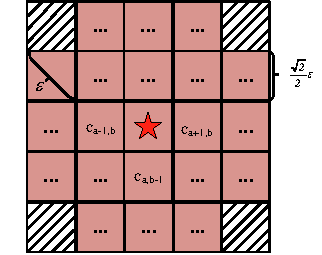
\includegraphics[width=0.6\textwidth]{fig/section5/cells.pdf}
    \caption{Potential cases of exposure}
    \label{fig:group}
\end{figure}
\paragraph{预检查策略。}
为了发现非查询组 $\mathcal{O}_{c'}$ 中所有与查询组 $\mathcal{O}_c^q$ 发生近距离接触的对象，直接计算需要 $O(|\mathcal{O}_c^q| \times |\mathcal{O}_{c'}|)$ 的时间复杂度，开销较大。为此，我们基于分组划分设计了若干预检查策略，以避免不必要的计算。具体而言，我们首先扫描 $\mathcal{O}_c^q$ 和 $\mathcal{O}_{c'}$ 中的所有位置点，分别得到其最小外包矩形 $\mathit{MBR}(\mathcal{O}_c^q)$ 和 $\mathit{MBR}(\mathcal{O}_{c'})$。公式 \ref{eq:pre-check} 定义了集合 $\{dist(l^{o_i}, l^{o_j}) \mid o_i \in \mathcal{O}_c^q, o_j \in \mathcal{O}_{c'}\}$ 的上界 $UB$ 和下界 $LB$。与 Hausdorff 距离相比，该预检查过程仅需要 $O(|\mathcal{O}_c^q| + |\mathcal{O}_{c'}|)$ 的线性时间复杂度。当上界 $UB(\mathcal{O}_c^q, \mathcal{O}_{c'})$ 小于 $\epsilon$ 时，我们可直接将 $\mathcal{O}_{c'}$ 中的所有对象视为近距离接触对象；相反，当下界 $LB(\mathcal{O}_c^q, \mathcal{O}_{c'}) > \epsilon$ 时，则可以安全地剪枝 $\mathcal{O}_{c'}$。

\begin{equation}
    \label{eq:pre-check}
        \begin{aligned}
        UB(\mathcal{O}_c^q, \mathcal{O}_{c'}) = \max (dist(\mathit{MBR}(\mathcal{O}_c^q), \mathit{MBR}(\mathcal{O}_{c'})))\\
        LB(\mathcal{O}_c^q, \mathcal{O}_{c'}) = \min (dist(\mathit{MBR}(\mathcal{O}_c^q), \mathit{MBR}(\mathcal{O}_{c'})))
        \end{aligned}
    \end{equation}

    \begin{algorithm}[!h]
        \caption{精确群体处理（EGP）算法}
        \label{alg:EGP}
        
        \Input{
        对象集合 $\mathcal{O}$；\newline
        位置流 $L_t(\mathcal{O}), L_{t+1}(\mathcal{O}), \ldots$；\newline
        查询对象集合 $\mathcal{Q} \subseteq \mathcal{O}$；\newline
        社交距离阈值 $\epsilon$；\newline
        接触时长阈值 $k$。
        }
        \Output{
        更新后的查询对象集合 $\mathcal{Q}$。
        }
        
        \textbf{初始化:}
        $\forall o \in (\mathcal{O} - \mathcal{Q})$: $cd(o) \leftarrow 0$；\newline
        $\Pi \leftarrow \emptyset$；$A \leftarrow \emptyset$；
        
        \For(\tcc*[f]{对象位置映射到网格}){each location $l_t^o \in L_t(\mathcal{O})$ of object $o$}{
            令 $c$ 为覆盖位置 $l_t^o$ 的网格单元；
        
            \If{$o \in \mathcal{Q}$}{
                $\Pi \leftarrow \{\Pi, c\}$；
                $\mathcal{O}_c^q \leftarrow \{\mathcal{O}_c^q, o\}$；
            }
            \Else{
                $\mathcal{O}_c \leftarrow \{\mathcal{O}_c, o\}$；
            }
        }
        
        \For(\tcc*[f]{处理查询单元}){each query cell $c \in \Pi$}{
            \For(\tcc*[f]{检查相邻非查询单元}){each non-query cell $c' \in SC(c)$}{
                \If{$UB(\mathcal{O}_c^q, \mathcal{O}_{c'}) \leq \epsilon$}{
                    $A \leftarrow \{A, \mathcal{O}_{c'}\}$；
                }
                \ElseIf{$LB(\mathcal{O}_c^q, \mathcal{O}_{c'}) \leq \epsilon$}{
                    $A \leftarrow \{A, ET(\mathcal{O}_c^q, \mathcal{O}_{c'})\}$；
                }
            }
        }
        
        更新 $cd(o)$；
        
        $\mathcal{Q} \leftarrow \{\mathcal{Q} \cup o \mid cd(o) \geq k\}$；
        
        \textbf{return} 更新后的 $\mathcal{Q}$；\tcp*[f]{实时结果}
        \end{algorithm}
    
        \paragraph{算法细节。}
        算法 \ref{alg:EGP} 给出了我们提出的精确群体处理（Exact Group Processing, EGP）算法的伪代码。其输入包括：对象集合 $\mathcal{O}$，位置流 $L_t(\mathcal{O})=\{l_t^o \mid o\in \mathcal{O}\}$（表示在每个时间戳 $t$ 时对象集合 $\mathcal{O}$ 的位置），查询对象集合，社交距离阈值 $\epsilon$，以及接触时长阈值 $k$。输出为更新后的查询对象集合，其中包含最新的暴露案例。
        
        在初始化阶段，所有非查询对象的接触时长 $cd(o)$ 被设置为 0（第 1 行）。在搜索过程中，我们使用 $\Pi$ 来存储至少覆盖一个查询对象的网格单元。同时，用 $A$ 表示当前发现的近距离接触对象集合。在算法开始时，$\Pi$ 和 $A$ 均被初始化为空集（第 2 行）。
        
        该算法包含两个阶段：1）群体划分阶段（第 3--11 行）；2）基于群体的近距离接触发现阶段（第 12--20 行）。在群体划分阶段，对于每一个到达的位置 $l_t^o$（对应对象 $o$），首先确定覆盖该位置的网格单元 $c$。如果 $o$ 是查询对象，则将其存入查询群体 $\mathcal{O}_c^q$，并将单元 $c$ 加入 $\Pi$；否则，将 $o$ 存入非查询群体 $\mathcal{O}_c$（第 3--11 行）。至此，所有查询群体和非查询群体均已构建完成。
        
        在近距离接触发现阶段，我们针对每一个查询群体及其相邻、具有潜在暴露风险的非查询群体，执行预检查策略（第 12--20 行）。具体而言，如果查询群体 $\mathcal{O}_c^q$ 与非查询群体 $\mathcal{O}_{c'}$ 之间距离的上界（参见公式 \ref{eq:pre-check}）不大于阈值 $\epsilon$，则将 $\mathcal{O}_{c'}$ 中的所有对象 $o$ 加入当前近距离接触集合 $A$。相反，如果其下界超过 $\epsilon$，则可以安全地剪枝 $\mathcal{O}_{c'}$，因为该群体中的任何对象都不可能与查询群体中的对象形成近距离接触。
        
        在完成群体级别的发现之后，我们进一步计算每个查询群体与其相邻、具有潜在暴露风险的非查询群体之间对象的成对距离（第 17 行）。在每一轮处理结束时，我们更新所有对象的接触时长（第 21 行）。具体地，对于所有不属于 $A$ 的对象 $o \in \mathcal{O} \setminus A$，将其接触时长重置为 0，表示在其接触时长达到阈值 $k$ 之前发生了中断。
        
        随后，对集合 $A$ 中的对象（即最新发现的近距离接触对象）更新其接触时长，并据此更新查询集合 $\mathcal{Q}$，将接触时长满足 $cd(o) \geq k$ 的对象作为最新的暴露案例加入其中（第 22 行）。最后，输出更新后的 $\mathcal{Q}$ 作为实时结果（第 23 行）。
        
        \paragraph{时间复杂度分析。}
        构建所有查询群体和非查询群体的时间复杂度为 $O(|\mathcal{O}|)$。设 $p$ 和 $q$ 分别表示每个查询群体和每个非查询群体中的对象数量，则发现近距离接触的时间复杂度为
        $O(|\Pi| \times |SC| \times p \times q)=O(|\Pi| \times p \times q)$，
        其中 $|SC|$ 为常数（参见群体划分过程）。
        
        在最坏情况下，一个网格单元可能覆盖所有查询对象，而另一个网格单元覆盖所有非查询对象（例如 $|\Pi|=1, p=|\mathcal{Q}|, q=|\mathcal{O}|$）。由于 $|SC|$ 为常数，此时每一轮运行 $EGP$ 的时间复杂度为 $O(|\mathcal{Q}||\mathcal{O}|)$。需要指出的是，在大多数实际场景中，$p$ 和 $q$ 通常远小于 $|\mathcal{Q}|$ 和 $|\mathcal{O}|$。

        \section{近似分组处理算法}

        为进一步提升暴露案例发现的效率，我们提出了一种 \underline{近似分组处理}（\underline{A}pproximate \underline{G}roup \underline{P}rocessing，AGP）算法。本节将介绍所采用的近似策略及算法细节。
        
        \paragraph{首尾优先检查策略。}
        在相邻的两个时间戳之间，可能存在大量对象彼此靠近地移动，但其中大多数对象并不能在较长时间内持续同行。若一个非查询对象在其接触时长尚未达到阈值 $k$ 之前未能持续成为近距离接触对象，则该对象不可能成为暴露案例。基于这一观察，我们提出了首尾优先检查策略。与按时间顺序逐一发现近距离接触不同，我们首先计算 $A_t$（即“尾部”）与 $A_{t-k}$（即“头部”）的交集，以获得在时间戳 $t$ 仍可能存在近距离接触的候选对象，其中 $A_t$ 表示时刻 $t$ 的近距离接触集合。对于时间区间 $[t-k+1,\, t]$，我们只需在该交集结果中进一步查找近距离接触，从而显著提升空间和时间效率。

        \begin{algorithm}[tb]
            \caption{近似分组处理算法（AGP）}
            \label{alg:AGP}
            \Input{
            对象集合 $\mathcal{O}$；\newline
            位置流 $L_t(\mathcal{O}), L_{t+1}(\mathcal{O}), \ldots$；\newline
            查询对象集合 $\mathcal{Q} \subseteq \mathcal{O}$；\newline
            社交距离阈值 $\epsilon$；\newline
            接触持续时间阈值 $k$；\newline
            跳跃步长 $m$。
            }
            \Output{实时近似暴露结果（更新后的查询集合 $\mathcal{Q}$）。}
            
            \BlankLine
            \textbf{初始化：} 对所有 $o \in (\mathcal{O}\setminus\mathcal{Q})$，令 $cd'(o)\leftarrow 0$；
            
            \If(\tcc*[f]{仅在跳跃时间点进行处理}){$t \bmod m = 0$}{
                $\Pi \leftarrow \emptyset$；$A' \leftarrow \emptyset$；
            
                \ForEach(\tcc*[f]{分组阶段}){对象 $o$ 在时刻 $t$ 的位置 $l_t^o \in L_t(\mathcal{O})$}{
                    令 $c$ 为覆盖 $l_t^o$ 的网格单元；\\
                    \uIf(\tcc*[f]{查询对象}){$o \in \mathcal{Q}$}{
                        $\Pi \leftarrow \Pi \cup \{c\}$；\\
                        $\mathcal{O}_c^q \leftarrow \mathcal{O}_c^q \cup \{o\}$；
                    }
                    \Else(\tcc*[f]{非查询对象}){%
                        $\mathcal{O}_c \leftarrow \mathcal{O}_c \cup \{o\}$；
                    }
                }
            
                \ForEach(\tcc*[f]{近邻单元扫描}){查询单元 $c \in \Pi$}{
                    \ForEach{非查询单元 $c' \in SC(c)$}{
                        $A' \leftarrow A' \cup \mathcal{O}_{c'}$；
                    }
                }
            
                \tcp{更新接触持续时间}
                更新所有对象的 $cd'(o)$；
            
                \tcp{头尾优先检查并更新查询集合}
                $\mathcal{Q} \leftarrow \mathcal{Q} \cup 
                \{\, o \mid o \in A_t \cap A_{t-k+1} \land cd'(o) \ge k \,\}$；
            }
            
            \textbf{return} 更新后的 $\mathcal{Q}$ 作为实时近似结果；
            \end{algorithm}

            \paragraph{跳跃检查。}
            给定接触时长阈值 $k$，若对象 $o$ 在连续 $k$ 个时间段 $[t_i, t_{i+k-1}]$ 内是潜在的暴露案例，并且在时间戳 $t_i$ 和 $t_{i+k-1}$ 均与至少一个查询对象发生近距离接触，则我们将对象 $o$ 视为一个近似暴露案例。
            基于近似暴露案例的定义，我们提出跳跃检查策略：
            不同于处理所有时间戳上的位置数据，我们仅在部分时间戳 $T=0,m,2m,\ldots$ 上处理位置数据，其中 $m$ 为跳跃长度。需要注意的是，当 $m=1$ 时，需要在每一个时间戳上进行处理。
            若时间戳 $t \notin T$，我们假设所有对象均为近距离接触对象。跳跃检查的目标是在不产生漏检的前提下，进一步降低计算开销。
            
            \paragraph{算法细节。}
            
            算法~\ref{alg:app} 给出了 AGP 算法的伪代码。与 EGP 相比，AGP 额外引入了跳跃长度 $m$ 作为输入参数。
            算法的输出为更新后的查询对象集合，其中包含原有查询对象以及最新发现的近似暴露案例。
            我们使用 $cd'(o)$ 表示对象 $o$ 作为潜在暴露案例的持续时长，并在算法开始时对每个非查询对象初始化 $cd'(o)$（第 1 行）。
            在算法中，仅当 $t \% m = 0$ 时，才在该时间戳上检测潜在暴露案例（第 2 行）。我们使用 $\Pi$ 来存储至少包含一个查询对象 $o\in \mathcal{Q}$ 的网格单元集合。
            我们分别用 $A$ 和 $A'$ 表示近距离接触集合和潜在暴露案例集合。
            对于对象 $o$ 在时间 $t$ 的位置 $l_t^o \in L_t(\mathcal{O})$，我们执行与 EGP 相同的操作以获得查询分组 $\mathcal{O}_c^q$ 以及非查询分组 $\mathcal{O}_c$（第 4--12 行）。
            随后，我们将位于 $SC(c)$ 中的对象视为潜在暴露案例，并相应地增加其接触时长（第 13--17 行）。
            接着，我们对不属于 $A'$ 的对象 $o$ 重置其接触时长（第 18 行）。
            对于满足 $cd'(o)\geq k$ 的对象，我们进一步检查其在时间戳 $t$ 和 $t-k+1$ 是否为近距离接触对象。若条件成立，则将其视为近似暴露案例，并将其加入查询集合 $\mathcal{Q}$（第 19 行）。
            最后，返回更新后的 $\mathcal{Q}$ 作为实时检测结果。
            
            \paragraph{时间复杂度分析。}
            分组划分过程需要 $O(|\mathcal{O}|)$ 的时间复杂度，主要差异体现在暴露案例的发现阶段。
            此外，潜在暴露案例的发现需要 $O(|\Pi|\times |SC|)=O(|\Pi|)$ 的时间。
            在最坏情况下，任意两个查询对象位于不同的网格单元中，即 $|\Pi|=|\mathcal{Q}|$。
            因此，AGP 算法每一轮的整体时间复杂度为 $O(|\mathcal{O}|+|\mathcal{Q}|)$。需要注意的是，$|\Pi|$ 的最大值为 $|\mathcal{Q}|$。

            

\section{实验研究}

\subsection{实验设置}

\paragraph{数据准备。}
我们的实验基于两个真实世界的轨迹数据集开展。第一个数据集来源于北京出租车数据集 \cite{DBLP:conf/kdd/YuanZXS11}，
包含在北京一周内跟踪到的 10,357 辆出租车的轨迹，总数据点数量约为 1,500 万。
第二个数据集采集自葡萄牙波尔图市（PT），时间跨度为 19 个月，包含超过 170 万条轨迹。
在北京数据集中，平均采样时间间隔为 177 秒，对应的平均移动距离约为 623 米；
而在波尔图数据集中，每辆出租车以 15 秒的间隔上报其位置信息。
时间戳的取值范围被限制在 24 小时之内。
我们限制经纬度范围，以保证采样位置具有足够高的空间密度。
此外，我们过滤掉采样点数量较少的轨迹，具体而言，仅保留采样点数量不少于 10 的轨迹用于实验。
为了能够在任意时间点计算对象（如出租车、行人）之间的距离，
我们通过线性插值对所有轨迹进行时间对齐，使得每个对象以固定频率返回其实时位置，
其中北京和波尔图数据集的频率分别为 10 秒和 5 秒。
最终，北京和波尔图数据集中分别包含 296,364,033 和 23,767,470 个有效位置点。
在不失一般性的前提下，我们从 $\mathcal{O}$ 中随机选取部分对象 $Q$ 作为初始查询对象。

\paragraph{对比算法。}
我们对比评估了所提出的算法，包括精确遍历算法（ET）、精确分组处理算法（EGP）以及近似算法（AGP）。
对于 AGP，默认的跳跃长度（hop length）设置为 2。
效率评估和效果评估所采用的性能指标分别为 CPU 时间以及发现的（近似）暴露案例总数。
为简化描述，我们使用 $|CE|$ 表示（近似）暴露案例的数量。
CPU 时间定义为每一轮算法运行的平均执行时间。
此外，我们还评估了 AGP 的准确性，其计算方式为真实暴露案例数量与近似暴露案例数量之比。

\paragraph{参数设置。}
默认参数设置如表 \ref{tb:para} 所示，该设置基于两个数据集的具体数据分布。
所有算法均采用 Java 实现，并在配备 AMD Ryzen 5 处理器（3.6GHz）和 32GB 内存的 Windows 10 平台上进行评测。
除非另有说明，实验结果均为在不同查询对象输入条件下进行 20 次独立实验后的平均值。
\begin{table}[tb]
    \centering
    \renewcommand\arraystretch{1.2}
    \begin{tabular}{l|rr}
    \toprule
        &\textbf{北京（Beijing）}&\textbf{波尔图（Porto）}\\
    \hline
    \hline
        经度 & [116.250, 116.550] & [-8.735, -8.156] \\
    \hline
        纬度 & [39.830, 40.030] & [40.953, 41.307] \\
    \hline
        $\epsilon$ & \{2, 4, 6, 8, 10\} & \{2, 4, 6, 8, 10\}  \\ 
        & 2 米（默认） & 2 米（默认） \\
    \hline
        $k$ & \{5, 10, 15, 20, 25\} & \{5, 7, 9, 11\} \\
        & 15（默认） & 5（默认） \\
    \hline
        $|\mathcal{Q}|$ & \{2, 4, 6, 8, 10\} $\times 10^2$  & \{2, 4, 6, 8, 10\} $\times 10^4$ \\
           & 600（默认） & 100{,}000（默认） \\
    \bottomrule
    \end{tabular}
    \caption{参数设置}
    \label{tb:para}
\end{table}

\subsection{性能评估}
\begin{figure}[tb]
    \centering
	\subfloat[北京]{
		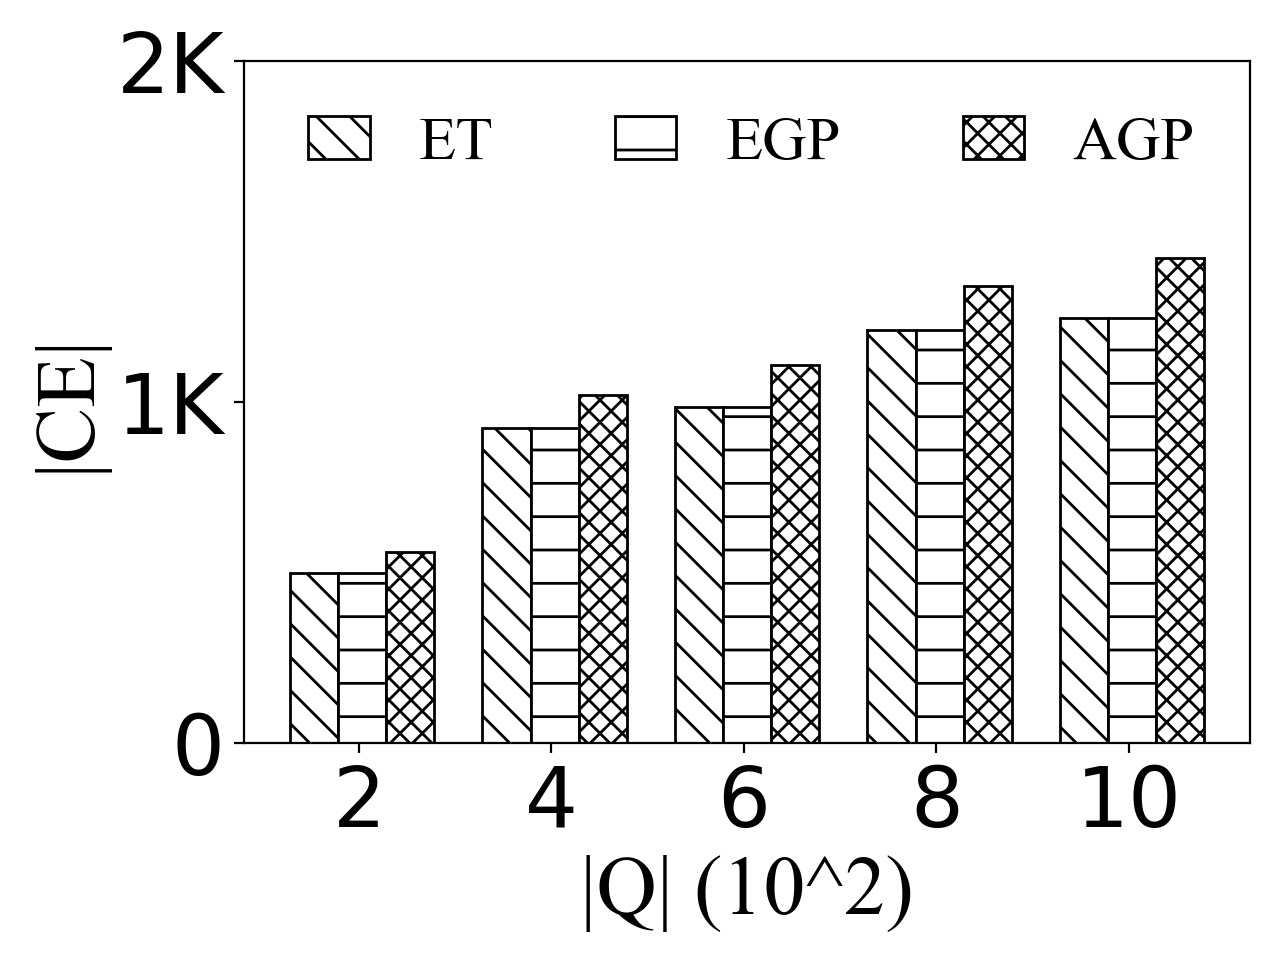
\includegraphics[width=0.4\textwidth]{fig/section5/BJ-Q-CE.png}
        \label{Beijing-Q-CE}
	}% 
    \hfill
	\subfloat[北京]{
    	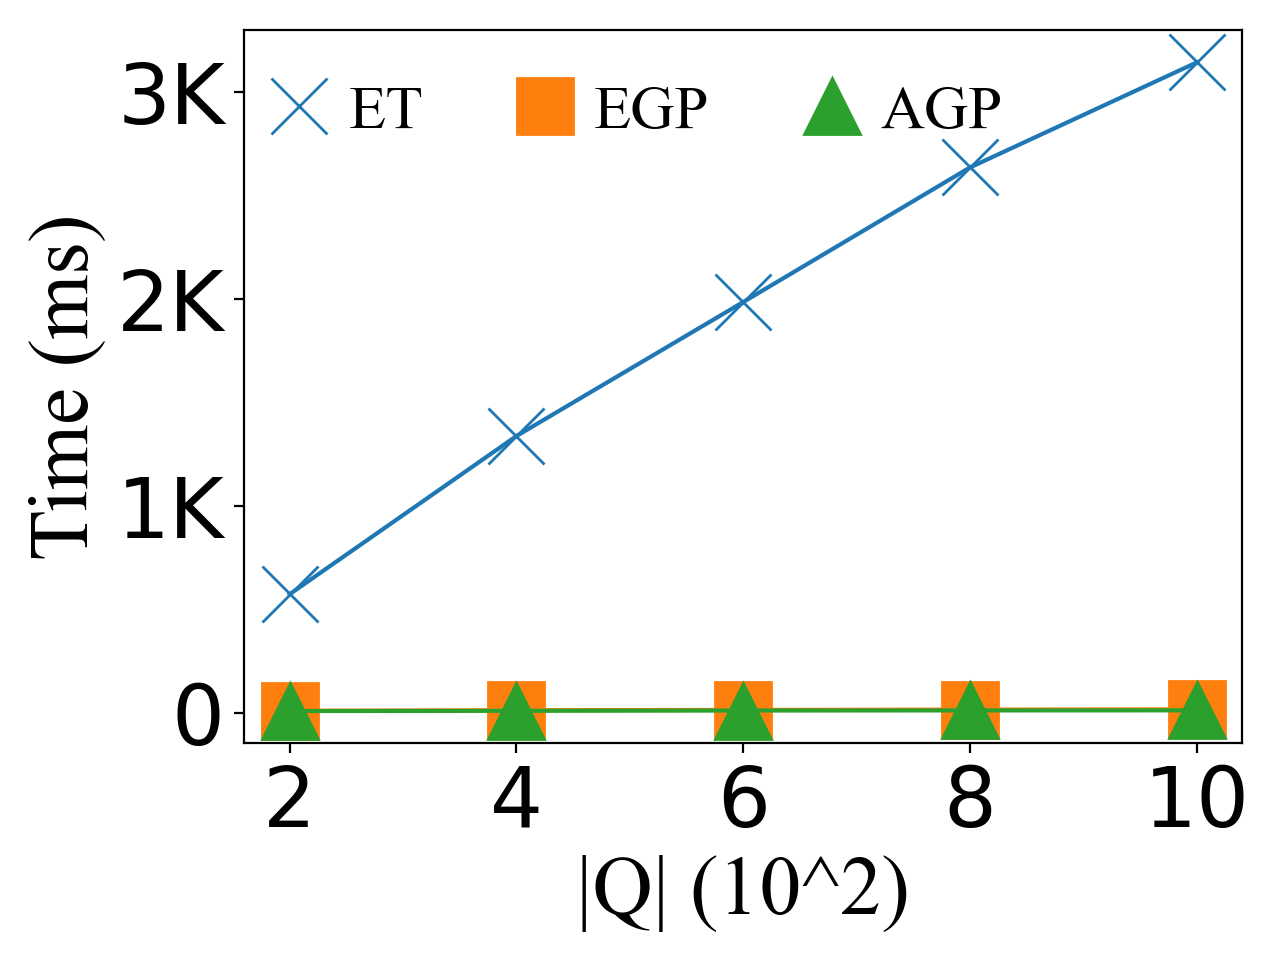
\includegraphics[width=0.4\textwidth]{fig/section5/BJ-Q-time.png}
    	\label{Beijing-Q-CPU}
	}%
	
	\subfloat[波尔图]{
		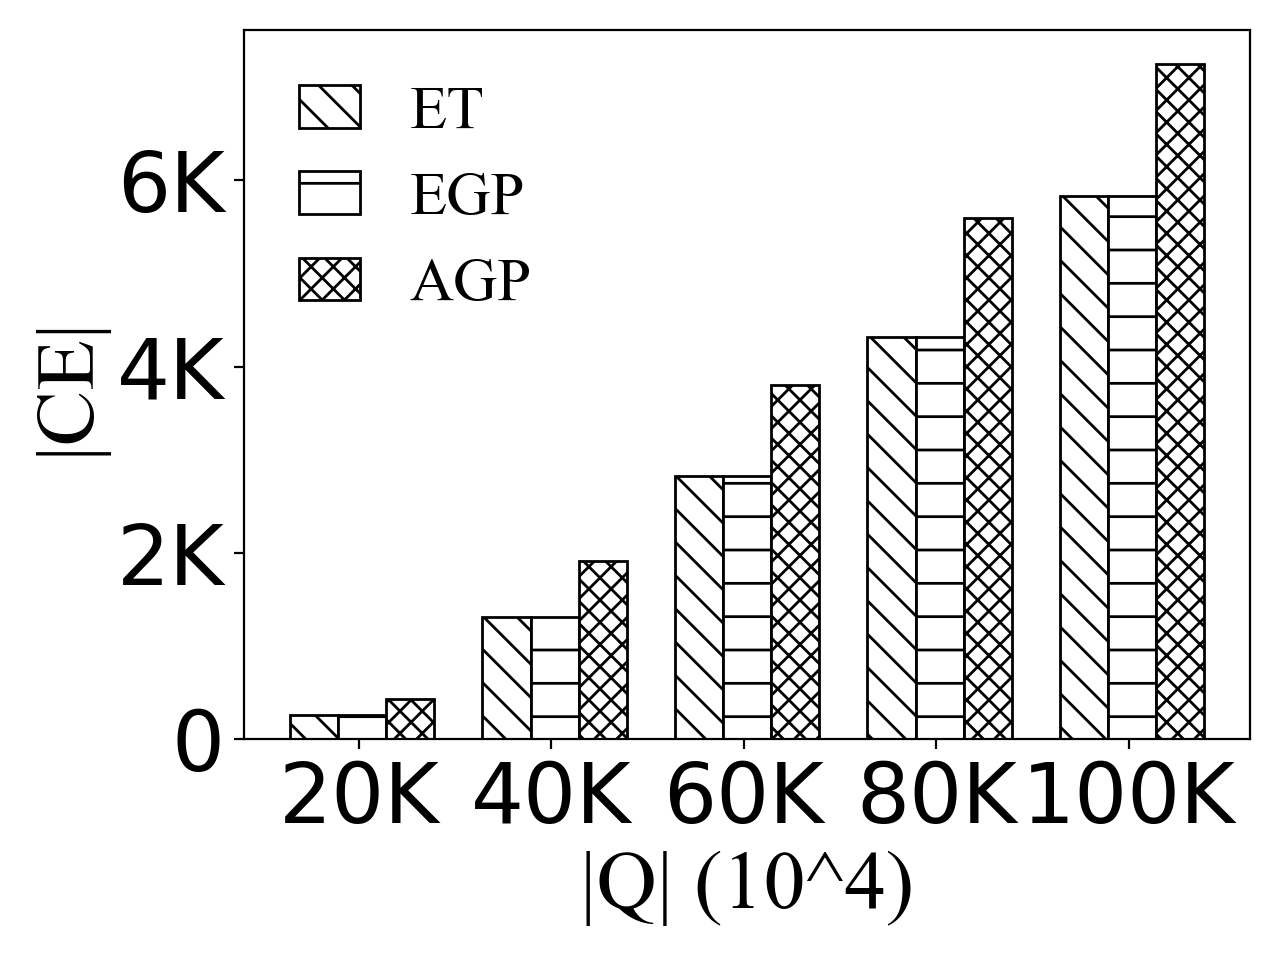
\includegraphics[width=0.4\textwidth]{fig/section5/PT-Q-CE.png}
		\label{Porto-Q-CE}
	}%
    \hfill
	\subfloat[波尔图]{
           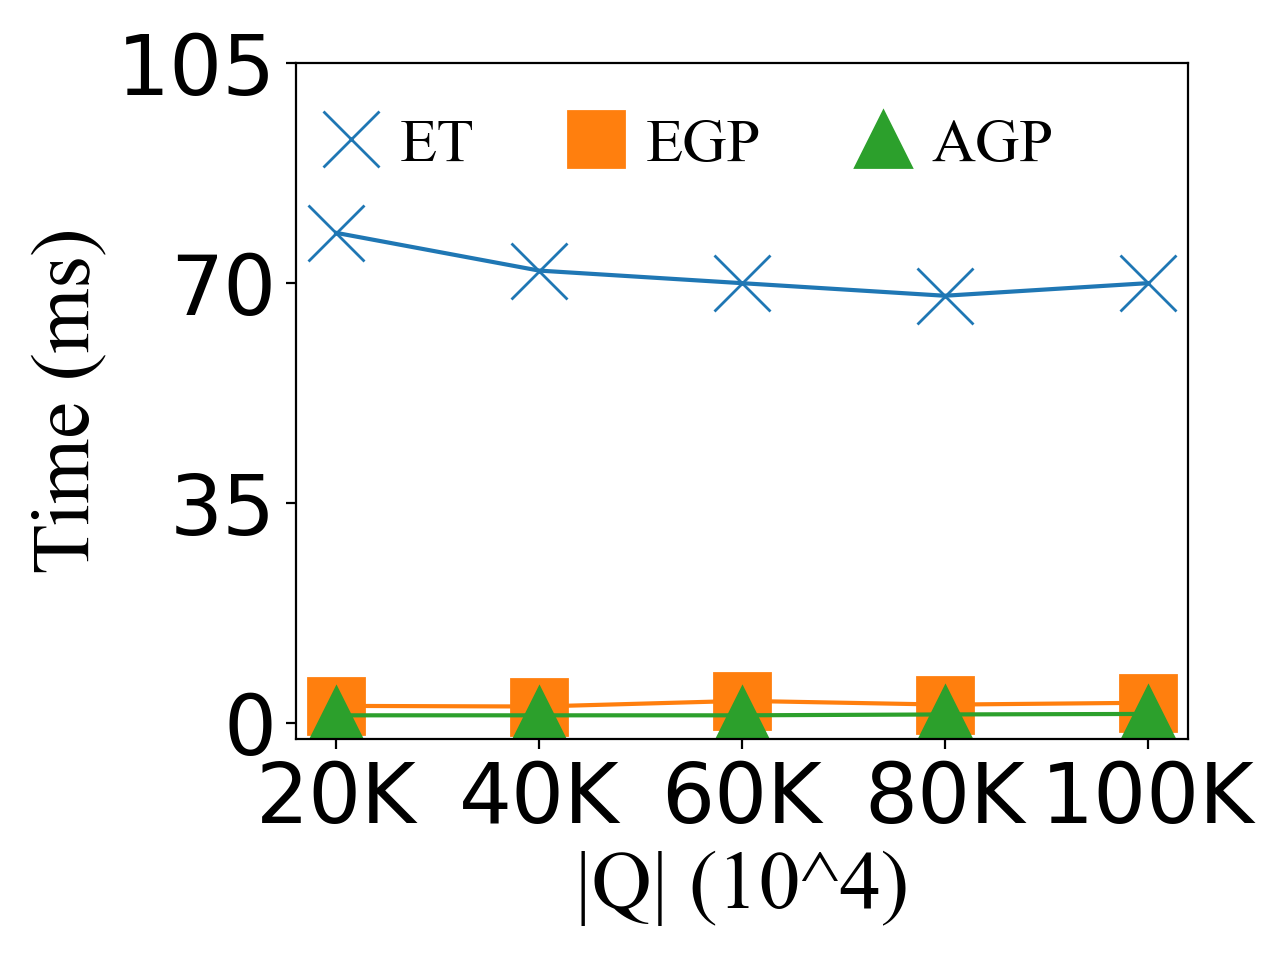
\includegraphics[width=0.4\textwidth]{fig/section5/PT-Q-time.png}
           \label{Porto-Q-CPU}
	}%
	\caption{查询对象数量的影响}
	\label{img:queryNum}
\end{figure}

\begin{figure}[htbp]
    \centering
	\subfloat[北京]{
		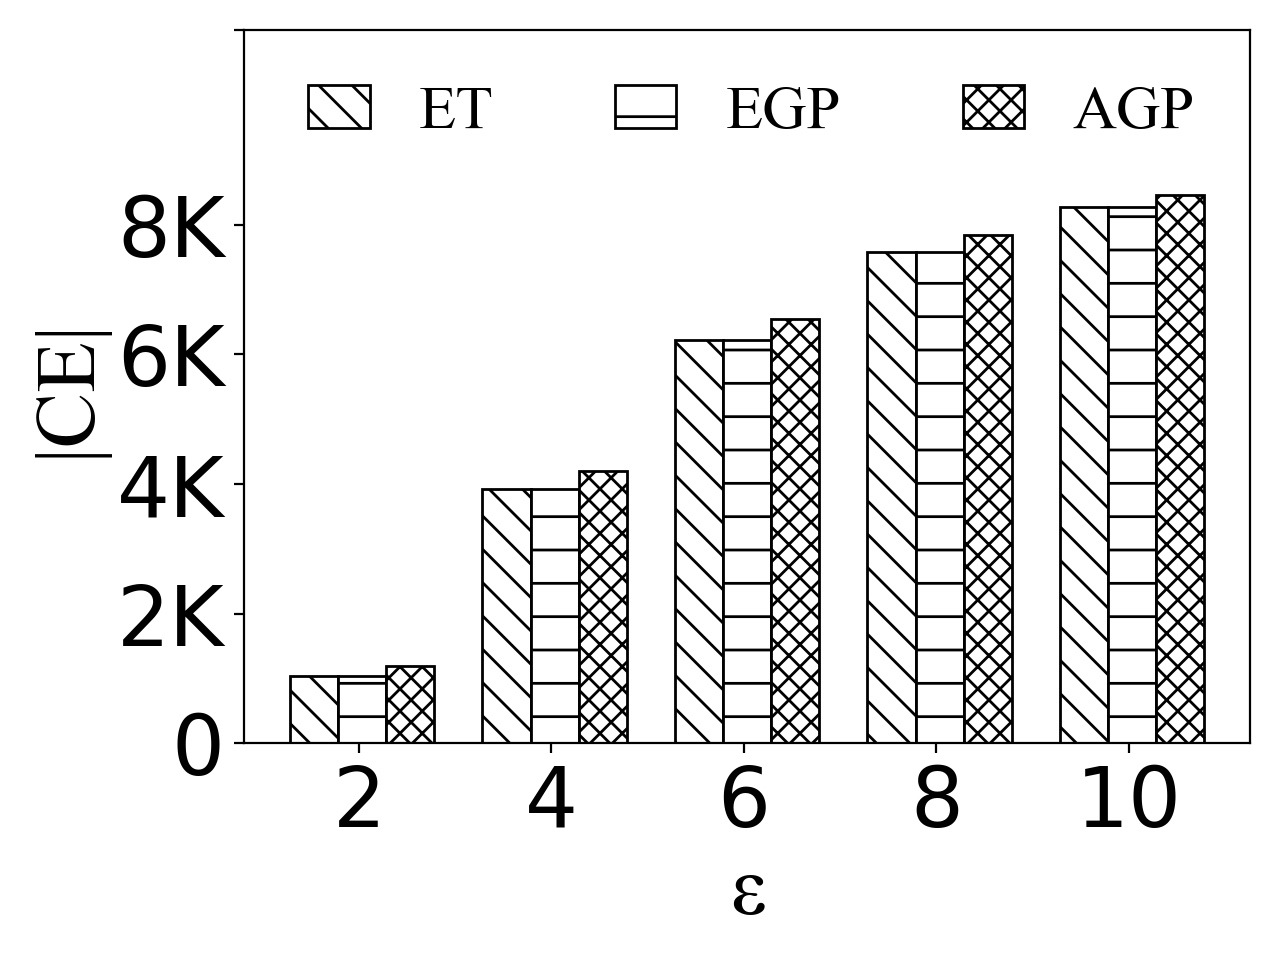
\includegraphics[width=0.4\textwidth]{fig/section5/BJ-ep-CE.png}
        \label{Beijing-ep-CE}
	}% 
    \hfill
	\subfloat[北京]{
    	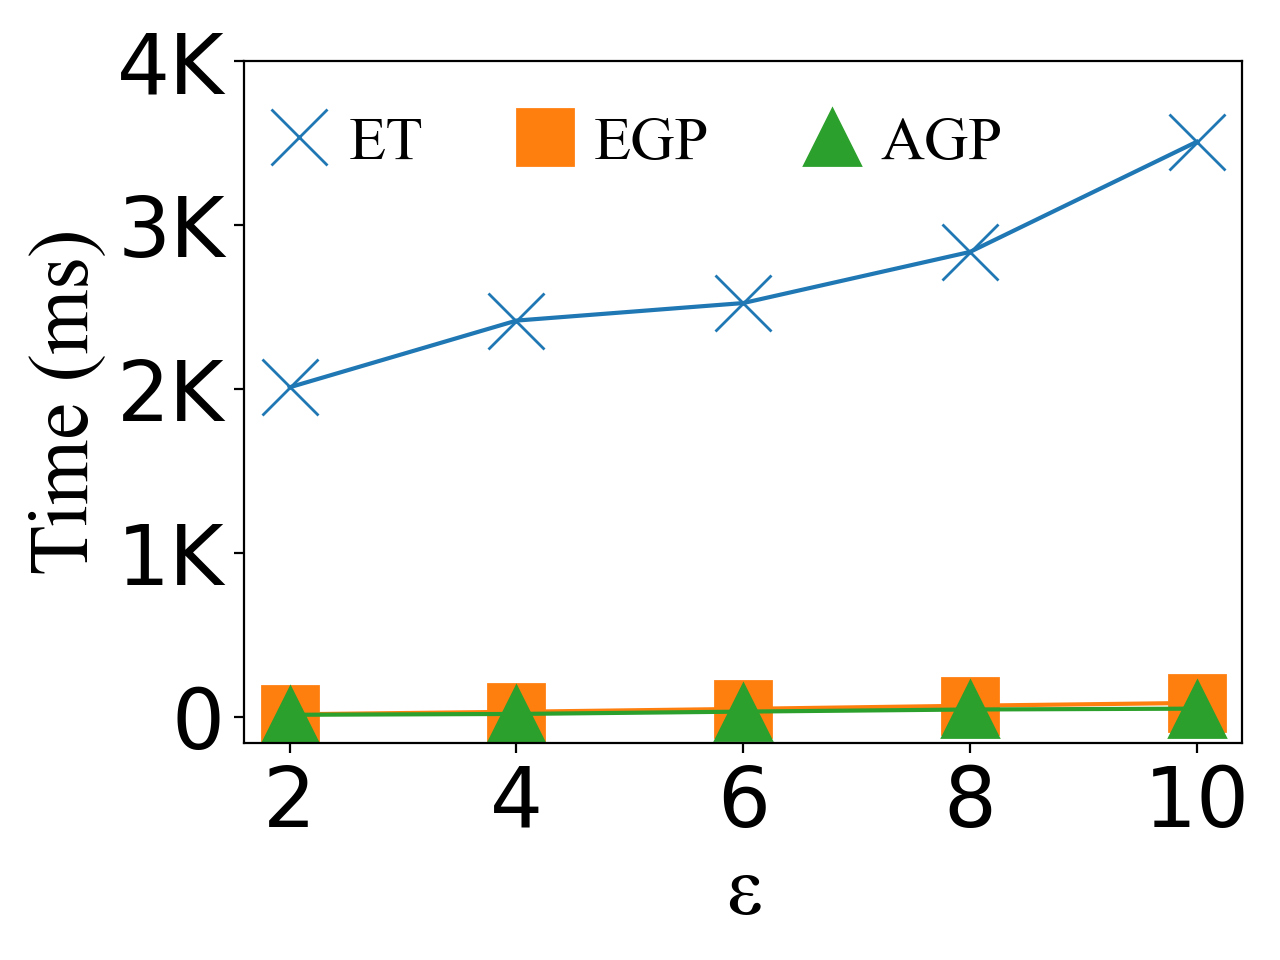
\includegraphics[width=0.4\textwidth]{fig/section5/BJ-ep-time.png}
    	\label{Beijing-ep-CPU}
	}%
	
	\subfloat[波尔图]{
		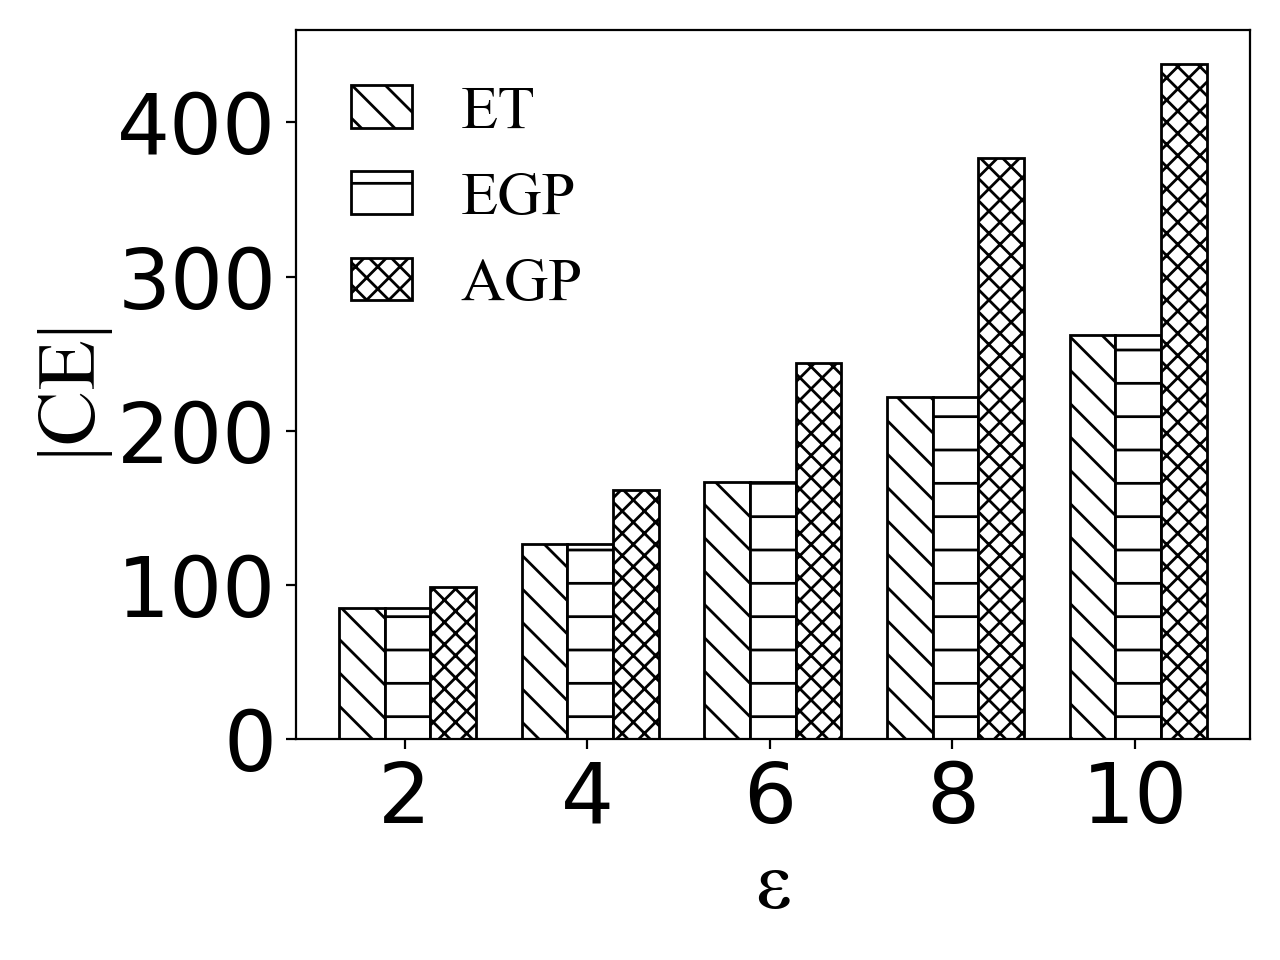
\includegraphics[width=0.4\textwidth]{fig/section5/PT-ep-CE.png}
		\label{Porto-ep-CE}
	}%
    \hfill
	\subfloat[波尔图]{
           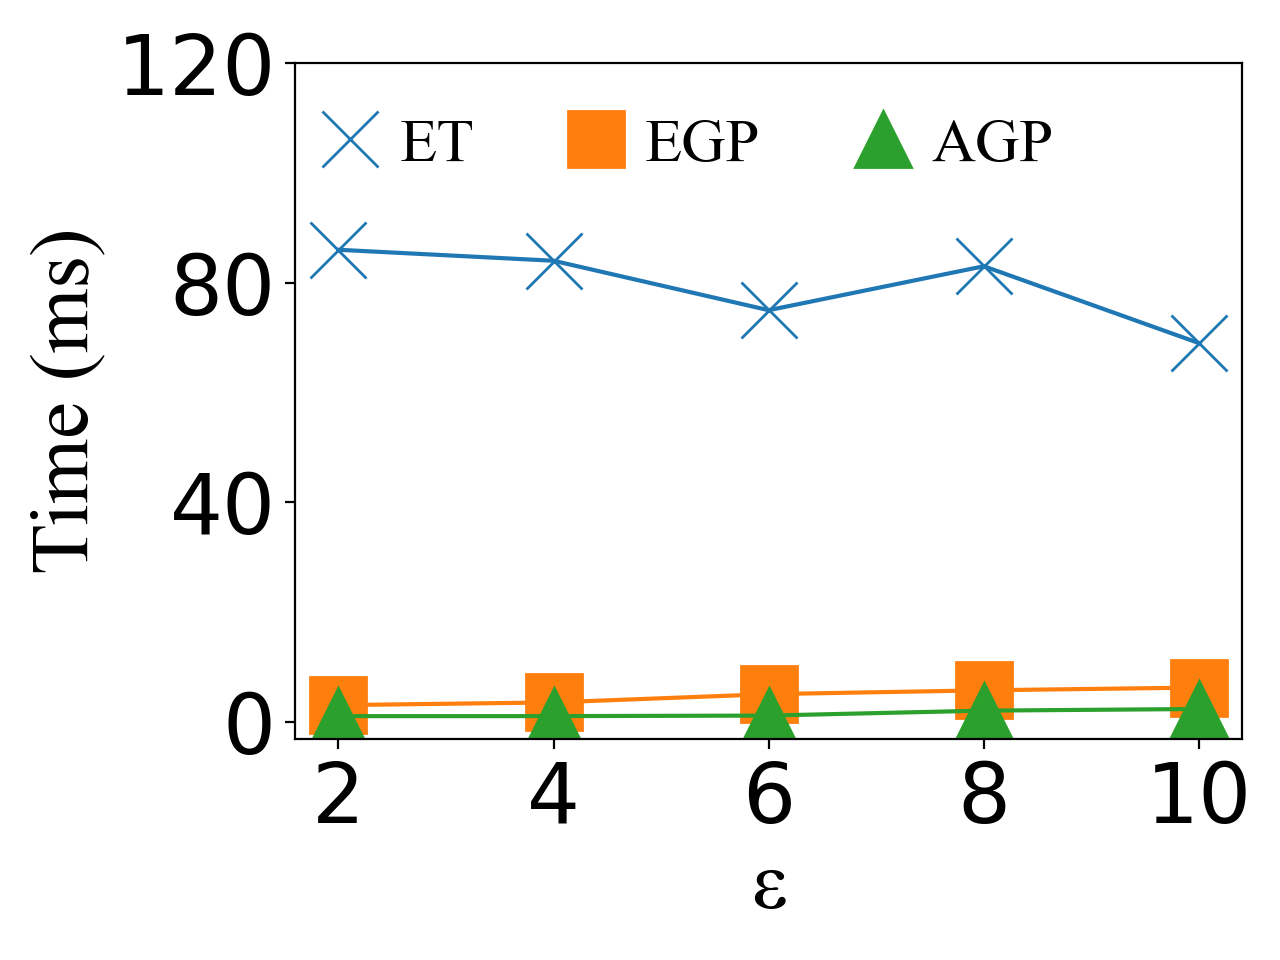
\includegraphics[width=0.4\textwidth]{fig/section5/PT-ep-time.png}
           \label{Porto-ep-CPU}
	}%
	\caption{距离阈值 $\epsilon$ 的影响}
	\label{img:ep}
\end{figure}


\paragraph{查询对象数量的影响。}
首先，我们在默认参数设置下研究查询对象数量 $|Q|$ 对所提出算法性能的影响。如图 \ref{Porto-Q-CE} 所示，在 Porto 数据集上，暴露案例数量呈现出显著的增长趋势，而在 BJ 数据集上该趋势并不明显。可以清楚地看到，ET 与 EGP 发现的暴露案例数量完全一致，这是因为它们都是精确算法。三种算法的结果总体上较为接近。如图 \ref{Beijing-Q-CPU} 和图 \ref{Porto-Q-CPU} 所示，在 CPU 时间方面，组处理算法的性能略逊于近似算法。ET 在处理北京数据集时所需的 CPU 时间超过 1{,}000 ms，这表明 ET 无法用于实时查询。相比之下，EGP 和 AGP 至少将所需 CPU 时间降低了一个数量级，充分体现了我们方法的优势。  

\paragraph{距离阈值 $\epsilon$ 的影响。}
直观上，较大的 $\epsilon$ 值意味着两个对象更容易与查询对象发生近距离接触。图 \ref{img:ep} 展示了当距离阈值 $\epsilon$ 从 2 米变化到 10 米时的性能表现。正如预期的那样，在 BJ 和 PT 数据集上，随着 $\epsilon$ 的增大，所有算法发现的暴露案例数量均随之增加。
从图 \ref{Beijing-ep-CE} 可以看出，在 BJ 数据集上，随着 $\epsilon$ 的增大，ET 与 AGP 结果之间的差异逐渐缩小；而在 PT 数据集上，这种差异则随着 $\epsilon$ 的增大而更加明显。这种现象可能归因于两种数据集在分布上的差异。值得注意的是，ET 算法的运行时间并没有呈现出明显的变化趋势，这是因为 ET 所需的计算开销在很大程度上依赖于查询对象的数量。  

\paragraph{接触持续时间 $k$ 的影响}
我们研究了接触持续时间阈值 $k$ 对算法性能的影响。较小的 $k$ 表示对象更容易被判定为暴露案例，从而导致暴露案例数量增加，并使得在每个时间快照下需要更高的 CPU 计算开销。如图 \ref{Beijing-k-CE} 和图 \ref{Porto-k-CE} 所示，当 $k$ 从 10 增加到 40 时，所有算法在北京和波尔图数据集上的暴露案例数量均显著下降。此外，从图 \ref{Beijing-k-CPU} 和图 \ref{Porto-k-CPU} 可以观察到 CPU 时间呈现出轻微的下降趋势，这是因为较大的 $k$ 会减少需要进一步检查的候选对象数量。

\paragraph{近似算法的评估}
图 \ref{img:app} 展示了在改变查询对象数量 $|Q|$ 和社交距离阈值 $\epsilon$ 时，AGP 算法的准确率表现。在北京数据集上，AGP 算法能够保持较高的准确率，并且在 $|Q|$ 和 $\epsilon$ 增加时未表现出明显的性能退化。相比之下，在波尔图数据集上，随着这些参数的增大，算法的准确率有所下降，这可能与不同数据集之间的分布特性和移动模式差异有关。

\paragraph{预检查策略的评估}
我们将不采用预检查策略的 EGP 方法记为 \textit{EGP*PC}。如图 \ref{img:precheck} 所示，在改变查询对象数量的情况下，EGP 在北京和波尔图数据集上的 CPU 时间始终低于 EGP*PC。这一结果清楚地表明，所提出的预检查策略能够有效减少不必要的计算开销，从而提升整体执行效率。

\section{本章小结}
我们提出并研究了一种新的暴露搜索问题，用于在轨迹位置流中发现暴露事件（CES 问题）。针对该问题，我们提出了两种高效算法，并设计了相应的预检查策略以提升整体计算效率。大量实验结果表明，所提出的方法在效率和有效性方面均表现优异，且预检查策略能够有效避免不必要的计算开销。